\documentclass[journal,12pt,twocolumn]{IEEEtran}

\usepackage{setspace}
\usepackage{gensymb}
\singlespacing
\usepackage[cmex10]{amsmath}

\usepackage{amsthm}

\usepackage{mathrsfs}
\usepackage{txfonts}
\usepackage{stfloats}
\usepackage{bm}
\usepackage{cite}
\usepackage{cases}
\usepackage{subfig}

\usepackage{longtable}
\usepackage{multirow}

\usepackage{enumitem}
\usepackage{mathtools}
\usepackage{steinmetz}
\usepackage{tikz}
\usepackage{circuitikz}
\usepackage{verbatim}
\usepackage{tfrupee}
\usepackage[breaklinks=true]{hyperref}
\usepackage{graphicx}
\usepackage{tkz-euclide}

\usetikzlibrary{calc,math}
\usepackage{listings}
    \usepackage{color}                                            %%
    \usepackage{array}                                            %%
    \usepackage{longtable}                                        %%
    \usepackage{calc}                                             %%
    \usepackage{multirow}                                         %%
    \usepackage{hhline}                                           %%
    \usepackage{ifthen}                                           %%
    \usepackage{lscape}     
\usepackage{multicol}
\usepackage{chngcntr}

\DeclareMathOperator*{\Res}{Res}

\renewcommand\thesection{\arabic{section}}
\renewcommand\thesubsection{\thesection.\arabic{subsection}}
\renewcommand\thesubsubsection{\thesubsection.\arabic{subsubsection}}

\renewcommand\thesectiondis{\arabic{section}}
\renewcommand\thesubsectiondis{\thesectiondis.\arabic{subsection}}
\renewcommand\thesubsubsectiondis{\thesubsectiondis.\arabic{subsubsection}}


\hyphenation{op-tical net-works semi-conduc-tor}
\def\inputGnumericTable{}                                 %%

\lstset{
%language=C,
frame=single, 
breaklines=true,
columns=fullflexible
}
\begin{document}


\newtheorem{theorem}{Theorem}[section]
\newtheorem{problem}{Problem}
\newtheorem{proposition}{Proposition}[section]
\newtheorem{lemma}{Lemma}[section]
\newtheorem{corollary}[theorem]{Corollary}
\newtheorem{example}{Example}[section]
\newtheorem{definition}[problem]{Definition}

\newcommand{\BEQA}{\begin{eqnarray}}
\newcommand{\EEQA}{\end{eqnarray}}
\newcommand{\define}{\stackrel{\triangle}{=}}
\bibliographystyle{IEEEtran}
\raggedbottom
\setlength{\parindent}{0pt}
\providecommand{\mbf}{\mathbf}
\providecommand{\pr}[1]{\ensuremath{\Pr\left(#1\right)}}
\providecommand{\qfunc}[1]{\ensuremath{Q\left(#1\right)}}
\providecommand{\sbrak}[1]{\ensuremath{{}\left[#1\right]}}
\providecommand{\lsbrak}[1]{\ensuremath{{}\left[#1\right.}}
\providecommand{\rsbrak}[1]{\ensuremath{{}\left.#1\right]}}
\providecommand{\brak}[1]{\ensuremath{\left(#1\right)}}
\providecommand{\lbrak}[1]{\ensuremath{\left(#1\right.}}
\providecommand{\rbrak}[1]{\ensuremath{\left.#1\right)}}
\providecommand{\cbrak}[1]{\ensuremath{\left\{#1\right\}}}
\providecommand{\lcbrak}[1]{\ensuremath{\left\{#1\right.}}
\providecommand{\rcbrak}[1]{\ensuremath{\left.#1\right\}}}
\theoremstyle{remark}
\newtheorem{rem}{Remark}
\newcommand{\sgn}{\mathop{\mathrm{sgn}}}
\providecommand{\abs}[1]{\(\left\vert#1\right\vert\)}
\providecommand{\res}[1]{\Res\displaylimits_{#1}} 
\providecommand{\norm}[1]{\(\left\lVert#1\right\rVert\)}
%\providecommand{\norm}[1]{\lVert#1\rVert}
\providecommand{\mtx}[1]{\mathbf{#1}}
\providecommand{\mean}[1]{E\(\left[ #1 \right]\)}
\providecommand{\fourier}{\overset{\mathcal{F}}{ \rightleftharpoons}}
%\providecommand{\hilbert}{\overset{\mathcal{H}}{ \rightleftharpoons}}
\providecommand{\system}{\overset{\mathcal{H}}{ \longleftrightarrow}}
	%\newcommand{\solution}[2]{\textbf{Solution:}{#1}}
\newcommand{\solution}{\noindent \textbf{Solution: }}
\newcommand{\cosec}{\,\text{cosec}\,}
\providecommand{\dec}[2]{\ensuremath{\overset{#1}{\underset{#2}{\gtrless}}}}
\newcommand{\myvec}[1]{\ensuremath{\begin{pmatrix}#1\end{pmatrix}}}
\newcommand{\mydet}[1]{\ensuremath{}}
\numberwithin{equation}{subsection}
\makeatletter
\@addtoreset{figure}{problem}
\makeatother
\let\StandardTheFigure\thefigure
\let\vec\mathbf
\renewcommand{\thefigure}{\theproblem}
\def\putbox#1#2#3{\makebox[0in][l]{\makebox[#1][l]{}\raisebox{\baselineskip}[0in][0in]{\raisebox{#2}[0in][0in]{#3}}}}
     \def\rightbox#1{\makebox[0in][r]{#1}}
     \def\centbox#1{\makebox[0in]{#1}}
     \def\topbox#1{\raisebox{-\baselineskip}[0in][0in]{#1}}
     \def\midbox#1{\raisebox{-0.5\baselineskip}[0in][0in]{#1}}
\vspace{3cm}
\title{AI1103 - Assignment 1}
\author{G Vojeswitha - AI20BTECH11024}
\maketitle
\newpage
\bigskip
\renewcommand{\thefigure}{\theenumi}
\renewcommand{\thetable}{\theenumi}
Download all python codes from 
\begin{lstlisting}
https://github.com/Vojeswitha05/Probability_AI1103/blob/main/Assignment_4/simulation_4.py
\end{lstlisting}
%
and latex-tikz codes from 
%
\begin{lstlisting}
https://github.com/Vojeswitha05/Probability_AI1103/blob/main/Assignment_4/latex_4.tex
\end{lstlisting}
\section{GATE EC, Q.23}
Two independent random variables \(X\) and \(Y\)
are uniformly distributed in the interval [-1,1].The probability that max [\(X\),\(Y\)] is less than \(\frac{1}{2}\) is
\begin{enumerate}[label={\Alph*)}]
    \item 3/4
    \item 9/16
    \item 1/4
    \item 2/3
\end{enumerate}
\section{Solution}
\begin{lemma}
 CDF of the random variable X is : 
 \begin{equation}
    F_X\brak{x}=
    \begin{cases}
    0 & x\leq-1\\
    \frac{1}{2}(x+1) & -1<x<1\\
    1 & x\geq1 
    \end{cases}\label{2.0.1}
 \end{equation}
\end{lemma}
\begin{proof}
Given X is uniformly distributed in [-1,1] i.e. X \(\sim\) U(-1,1)
\\PDF of X : 
\begin{equation}
    f_{X}\brak{x}=
    \begin{cases}
     0 & x\leq-1\\
     \frac{1}{2} & -1\leq x\leq 1\\
     0 & x\geq1
    \end{cases}
\end{equation}
For  \(-1\leq x\leq 1\)
\begin{align}
  F_{X}\brak{x}&=\Pr\brak{X\leq x}\\
  &=\int_{-1}^x\frac{1}{2}dx\\
  &=\frac{1}{2}(x+1)
\end{align}
Hence \eqref{2.0.1} is proved
\end{proof}
\begin{lemma}
 CDF of the random variable X is : 
 \begin{equation}
    F_X\brak{x}=
    \begin{cases}
    0 & x\leq-1\\
    \frac{1}{2}\brak{x+1} & -1<x<1\\
    1 & x\geq1 
    \end{cases}\label{2.0.5}
 \end{equation}
\end{lemma}
\begin{proof}
Given Y is uniformly distributed in [-1,1] i.e. Y \(\sim\) U(-1,1)
\\PDF of Y : 
\begin{equation}
    f_{Y}\brak{y}=
    \begin{cases}
     0 & y\leq-1\\
     \frac{1}{2} & -1\leq y\leq 1\\
     0 & y\geq1
    \end{cases}
\end{equation}
For  \(-1\leq y\leq 1\)
\begin{align}
  F_{Y}\brak{y}&=P(Y\leq y)\\
  &=\int_{-1}^y\frac{1}{2}dy\\
  &=\frac{1}{2}\brak{y+1}
\end{align}
Hence \eqref{2.0.5} is proved
\end{proof}
\begin{lemma}
\begin{align}
    \Pr\brak{{max\brak{X,Y}<\frac{1}{2}}} = \frac{9}{16}\label{2.0.11}
\end{align}
\end{lemma}
\begin{proof}
\({max\brak{X,Y}}<\frac{1}{2} \implies\) \(X<\frac{1}{2}\) \& \(Y<\frac{1}{2}\)\\
Given X and Y are independent,
\begin{align}
    Pr(X<\frac{1}{2},&Y<\frac{1}{2})\\
    &=\Pr\brak{X <\frac{1}{2}}\times \Pr\brak{Y <\frac{1}{2}}\\
    &=F_X\brak{\frac{1}{2}} \times F_Y\brak{\frac{1}{2}}\\
   &=\frac{3}{2}\times\frac{1}{2}\times\frac{3}{2}\times\frac{1}{2}\\
    &=\frac{9}{16}
\end{align}
Hence \eqref{2.0.11} is proved
\end{proof}
Option B is correct
\begin{figure}[h!]
    \centering
    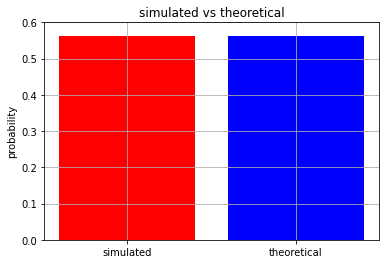
\includegraphics[width=12cm]{sim vs ther.png}
    \caption{simulated vs theoretical}
    \label{fig:my_label}
\end{figure}
\end{document}

